%% !TEX root = ../../handbook-physics.tex
%%!TEX TS-program = pdflatex
%%!TEX encoding = UTF-8 Unicode


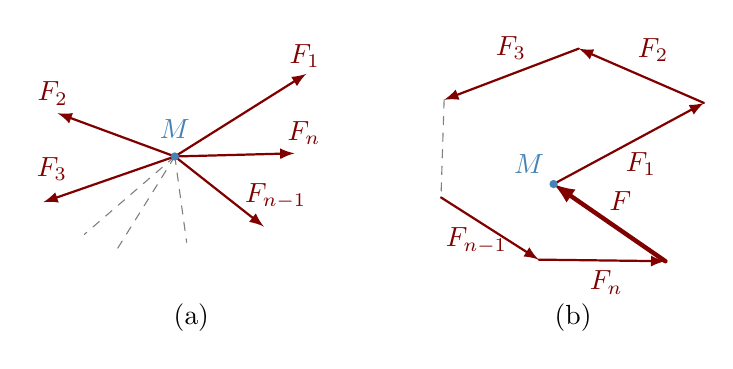
\begin{tikzpicture}[line cap=round,line join=round,scale=1]
\draw [thick,-latex,Maroon] (0.,0.)-- (1.67,1.05);
\draw [thick,-latex,Maroon] (0.,0.)-- (1.52,0.04);
\draw [thick,-latex,Maroon] (0.,0.)-- (1.13,-0.89);
\draw [dashed,color=gray] (0.,0.)-- (0.15,-1.09);
\draw [dashed,color=gray] (0.,0.)-- (-0.76,-1.22);
\draw [dashed,color=gray] (0.,0.)-- (-1.15,-0.99);
\draw [thick,-latex,Maroon] (0.,0.)-- (-1.67,-0.58);
\draw [thick,-latex,Maroon] (0.,0.)-- (-1.49,0.55);
\draw [thick,-latex,Maroon] (3.38,-0.52)-- (4.62,-1.31);
\draw [thick,-latex,Maroon] (4.62,-1.31)-- (6.23,-1.33);
\draw [ultra thick,-latex,Maroon] (6.23,-1.33)-- (4.81,-0.35);
\draw [thick,-latex,Maroon] (4.81,-0.35)-- (6.72,0.68);
\draw [thick,-latex,Maroon] (6.72,0.68)-- (5.13,1.37);
\draw [thick,-latex,Maroon] (5.13,1.37)-- (3.42,0.72);
\draw [dashed,color=gray] (3.42,0.72)-- (3.38,-0.52);
\draw (-0.14,-1.75) node[anchor=north west] {(a)};
\draw (4.70,-1.75) node[anchor=north west] {(b)};
\fill [fill=SteelBlue] (0.,0.) circle (1.5pt);
\draw[color=SteelBlue] (0,0.1) node [above]{$M$};
\draw[color=Maroon] (1.65,1.28) node {$\vb{F_{1}}$};
\draw[color=Maroon] (1.64,0.30) node {$\vb{F_{n}}$};
\draw[color=Maroon] (1.28,-0.5) node {$\vb{F_{n-1}}$};
\draw[color=Maroon] (-1.56,-0.16) node {$\vb{F_{3}}$};
\draw[color=Maroon] (-1.55,0.8) node {$\vb{F_{2}}$};
\draw[color=Maroon] (3.83,-1.07) node {$\vb{F_{n-1}}$};
\draw[color=Maroon] (5.48,-1.6) node {$\vb{F_{n}}$};
\fill [fill=SteelBlue] (4.81,-0.35) circle (1.5pt);
\draw[color=SteelBlue] (4.50,-0.10) node {$M$};
\draw[color=Maroon] (5.66,-0.57) node {$\vb{F}$};
\draw[color=Maroon] (5.92,-.1) node {$\vb{F_{1}}$};
\draw[color=Maroon] (6.073606961153187,1.3477958122999878) node {$\vb{F_{2}}$};
\draw[color=Maroon] (4.26875694360382,1.3723515948516798) node {$\vb{F_{3}}$};
\end{tikzpicture}
